%%%%%%%%%%%%%%%%%%%%%%%%%%%%%%%%%%%%%%%%%
% Dreuw & Deselaer's Poster
% LaTeX Template
% Version 1.0 (11/04/13)
%
% Created by:
% Philippe Dreuw and Thomas Deselaers
% http://www-i6.informatik.rwth-aachen.de/~dreuw/latexbeamerposter.php
%
% This template has been downloaded from:
% http://www.LaTeXTemplates.com
%
% License:
% CC BY-NC-SA 3.0 (http://creativecommons.org/licenses/by-nc-sa/3.0/)
%
%%%%%%%%%%%%%%%%%%%%%%%%%%%%%%%%%%%%%%%%%

%----------------------------------------------------------------------------------------
%	PACKAGES AND OTHER DOCUMENT CONFIGURATIONS
%----------------------------------------------------------------------------------------

\documentclass[final,hyperref={pdfpagelabels=false}]{beamer}

\usepackage[orientation=portrait,size=a0,scale=1.4]{beamerposter} % Use the beamerposter package for laying out the poster with a portrait orientation and an a0 paper size

\usetheme{I6pd2} % Use the I6pd2 theme supplied with this template

\usepackage[english]{babel} % English language/hyphenation

\usepackage{amsmath,amsthm,amssymb,latexsym} % For including math equations, theorems, symbols, etc

%\usepackage{times}\usefonttheme{professionalfonts}  % Uncomment to use Times as the main font
%\usefonttheme[onlymath]{serif} % Uncomment to use a Serif font within math environments

\boldmath % Use bold for everything within the math environment

\usepackage{booktabs} % Top and bottom rules for tables

\graphicspath{{figures/}} % Location of the graphics files

\usecaptiontemplate{\small\structure{\insertcaptionname~\insertcaptionnumber: }\insertcaption} % A fix for figure numbering

%----------------------------------------------------------------------------------------
%	TITLE SECTION 
%----------------------------------------------------------------------------------------

\title{\huge Experiments in Combining \\ Boosting and Deep Stacked Networks} % Poster title

\author{Manuel~Montoya-Catal\'{a}, Ricardo~F.~Alvear-Sandoval,
        An\'{i}bal~R.~Figueiras-Vidal} % Author(s)

\institute{Signal Theory and Communications Department of the Univ. Carlos III of Madrid} % Institution(s)

%----------------------------------------------------------------------------------------
%	FOOTER TEXT
%----------------------------------------------------------------------------------------

\newcommand{\leftfoot}{2016 IEEE International Workshop on Machine Learning for Signal Processing} % Left footer text

\newcommand{\rightfoot}{\tiny REF- 96149218249375386387392398419420435502} % Right footer text

%----------------------------------------------------------------------------------------

\begin{document}

\addtobeamertemplate{block end}{}{\vspace*{2ex}} % White space under blocks

\begin{frame}[t] % The whole poster is enclosed in one beamer frame

\begin{columns}[t] % The whole poster consists of two major columns, each of which can be subdivided further with another \begin{columns} block - the [t] argument aligns each column's content to the top

\begin{column}{.02\textwidth}\end{column} % Empty spacer column

\begin{column}{.465\textwidth} % The first column

%----------------------------------------------------------------------------------------
%	OBJECTIVES
%----------------------------------------------------------------------------------------

\begin{block}{Objectives}

\begin{enumerate}
\item To develop new Deep Learning architectures and training algorithms

\item To combine Deep Learning architectures with Boosting, creating systems with high expressivity and resistance to overfitting

\item To propose flexible emphasis functions that can moderate boosting

\end{enumerate}

\end{block}

%----------------------------------------------------------------------------------------
%	INTRODUCTION
%----------------------------------------------------------------------------------------
            
\begin{block}{Introduction}

Both boosting and deep stacking sequentially train their units taking into account the outputs of the previously trained learners. This parallelism suggests that it exists the possibility of getting some advantages by combining these widely known techniques, i.e., emphasis and injection, in appropiate manners. 
               
We propose a first mode for such a combination by simultaneously applying a general and flexible enough emphasis function and injecting the aggregated previous outputs to the learner which is being designed. We call this kind of classification mechanism Boosted and Aggregated Deep Stacked Networks (B-ADSNs).

\end{block}

\begin{block}{	Deep Stacked Networks (DSNs)}

DSNs are a family of Deep Learning architectures in which each unit (layer) consists of a MLP whose input is: 

\begin{itemize}
\setlength{\itemindent}{2em}

\item[--] The observed features and 
\item[--] The outputs of all previously trained learners
\end{itemize}
\centering
\begin{figure}
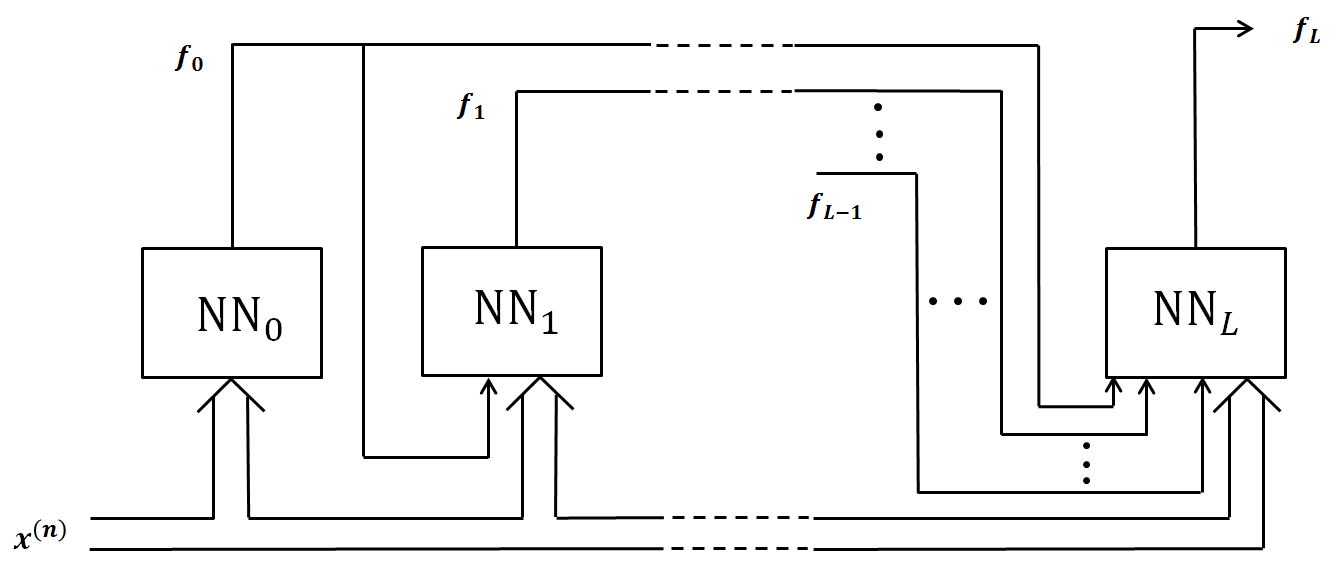
\includegraphics[width=0.75\linewidth]{DSNs1.png}
\caption{Deep Stacked Network architecture}
\end{figure}
\begin{itemize}
\setlength{\itemindent}{1em}
\item The output of the ensemble is the output of the last unit.
\item This architecture has a high expressivity but it is prone to overfitting.
\item The dimensionality of the input space increases with the number of units.
\end{itemize}
\end{block}

%----------------------------------------------------------------------------------------
%	Boosting
%----------------------------------------------------------------------------------------
\begin{block}{	Boosting}

Boosting is an ensemble method in which learners are sequentially trained using information from the aggregation of all previously trained units. 

\begin{itemize}
\setlength{\itemindent}{2em}
\item[--]  During the training of every unit, each sample is assigned an emphasis value $\mathit{e_{l}(x^{(n)})}$. The set of emphasis value generates a discrete distribution over the samples.
\item[--] This value indicates the "importance" of the sample during training. It weights its contribution to the loss function.
\item[--] The emphasis function assings this value to every sample according to their current error value. Samples that are easily classified by the system obtain low values of importance.
\end{itemize}

\centering
\begin{figure}
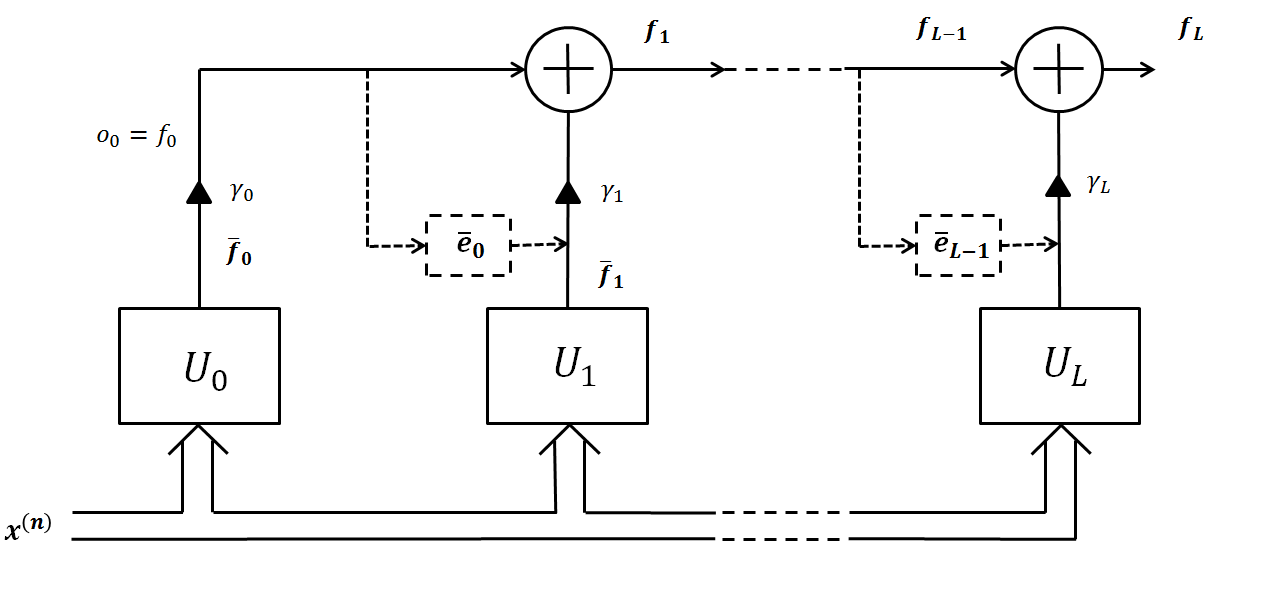
\includegraphics[width=0.8\linewidth]{Boost1.png}
\caption{Boosting architecture}
\end{figure}
\begin{itemize}
\setlength{\itemindent}{1em}
\item The output of the ensemble is a linear combination of all unit outputs.
\item Resistant to overfitting.
\item Boosting ensembles usually require weak learners.
\end{itemize}
\end{block}

--------------------------------
\end{column} % End of the first column

\begin{column}{.03\textwidth}\end{column} % Empty spacer column
 
\begin{column}{.465\textwidth} % The second column

\begin{block}{	Boosted Aggregated Deep Stacked Networks}

Combination of DSNs and Boosting by means of an aggregated output injection and a flexible emphasis function. Each unit has two additional sources of information:

\begin{itemize}
\setlength{\itemindent}{2em}
\item[--] Injection of the aggregated output of all previously trained units.
\item[--] Emphasis values of the samples.
\end{itemize}

\begin{figure}
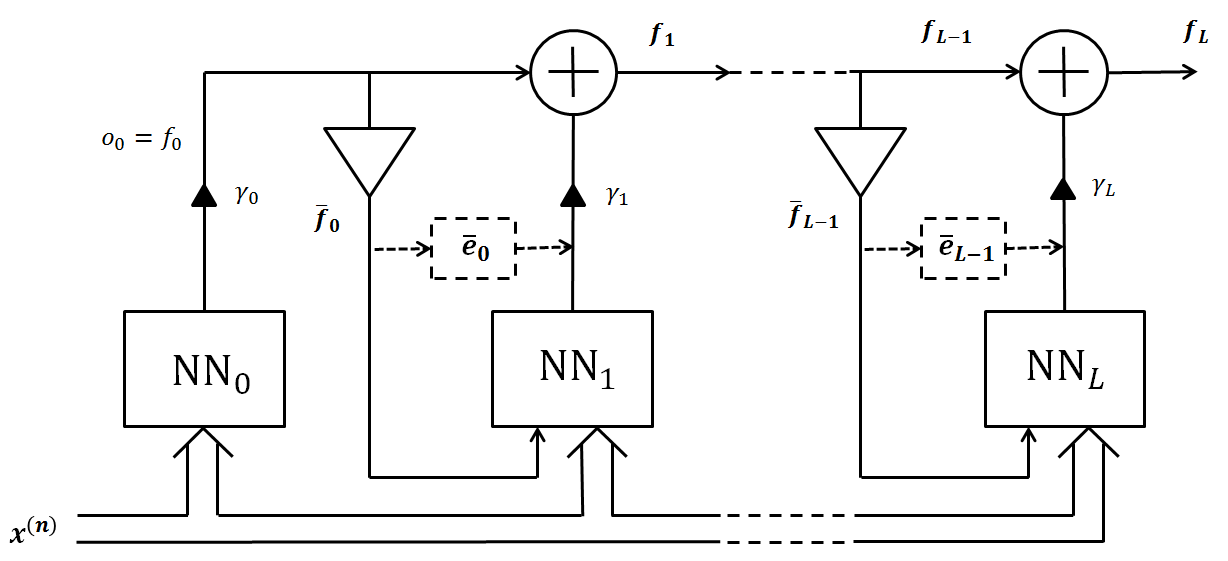
\includegraphics[width=0.8\linewidth]{BADSN1.png}
\caption{Boosted Aggregated Deep Stacked Networks architecture}
\end{figure}

\begin{itemize}
\item The emphasis function $e_{l}^*(\mathbf{x}^{(n)})$ constains the hyperparameters $\alpha$ and $\beta$ which control the intensity of the boosting so that the optimal combination of boosting and outputs' injection can be found.

\begin{equation}
\begin{split}
e_{l}^*(\mathbf{x}^{(n)}) = &\frac{\alpha }{N}  + \frac{1 - \alpha}{Z_{l}} \bigg[ e_{l}^* (\mathbf{x}^{(n)}) \cdot \\  
 \exp  \bigg( 
 & \beta \big( t^{(n)}- \overline{f}^{2}_{l-1} (\mathbf{x}^{(n)})\big)^2 - (1 - \beta)\overline{f}^{2}_{l-1} (\mathbf{x}^{(n)})   \bigg)\bigg] 
\end{split}
\end{equation}


\normalsize
\item The learners are trained using Online Backpropagation. 
\item The values of $\alpha$, $\beta$ and the hyperparameters of the architecture are obtained by means of crossvalidation (CV).

\end{itemize}

\end{block}

\begin{block}{Results}
The following table contains  the average error rate $\pm$ standard deviation for the considered architectures -- deep learning architectures B-ADSN including the restricted version ADSN, and the boosting ensemble B1. CV values for $\alpha$, $\beta$, $N_{ep}$ and $H$ are also included.
\begin{figure}
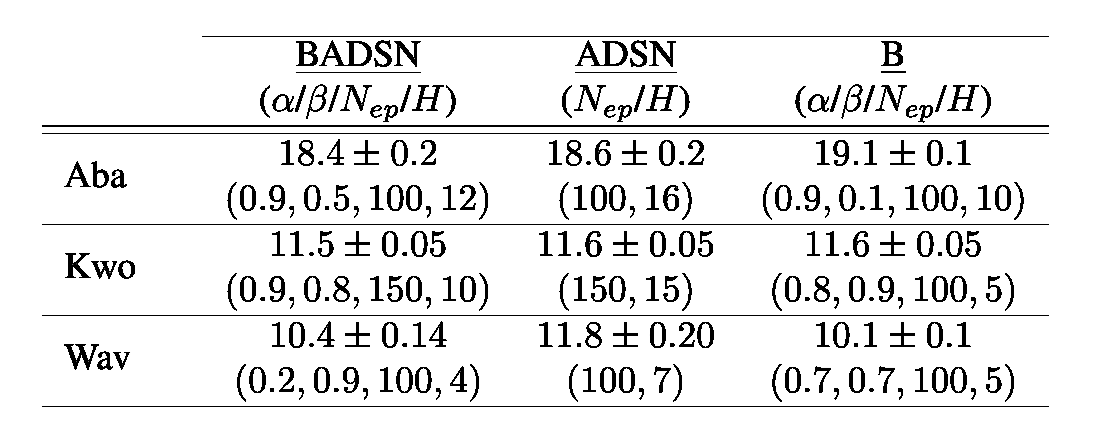
\includegraphics[width=0.8\linewidth]{table1.png}
\caption{Results Table}
\end{figure}
\begin{itemize}
\setlength{\itemindent}{1em}
\item The accuracy of the system varies smoothly with respect to the parameters $\alpha$ and $\beta$.
\item The performance of the system converges with the number of layers.

\end{itemize}
\end{block}

%------------------------------------------------


%----------------------------------------------------------------------------------------
%	CONCLUSION
%----------------------------------------------------------------------------------------

\begin{block}{Conclusions}

\begin{itemize}
\setlength{\itemindent}{0.5em}
\item The combination of the expressivity of DSNs and the resistance to overfitting of boosting can be succesfull.

\item A flexible emphasis function is required to moderate the boosting contribution.

\item There are many other possible combinations of boosting and deep learning.
\end{itemize}

\end{block}

%----------------------------------------------------------------------------------------
%	REFERENCES
%----------------------------------------------------------------------------------------

\begin{block}{References}
        
\nocite{*} % Insert publications even if they are not cited in the poster
\small{\bibliographystyle{unsrt}

[1] L.Deng and D.Yu, "Deep convex net: A scalable architecture for speech classification", in \textit{Proc. Interspeech 2011}, pp. 2285-2288. Florence (Italy), 2011.

[2] R. E. Schapire and Y. Freund. Boosting: Foundations and Algorithms. Cambridge, MA: MIT Press, 2012.

[3] V. G\'{o}mez-Verdejo, M. Ortega-Moral, J. Arenas-Garc\'{i}a and A. R. Figueiras-Vidal, "Boosting by weighting critical and erroneous samples", \textit{Neurocomputing}

[4] J. T.-Y. Kwok.  "Moderating the outputs of support vector machine classifiers"

\bibliography{sample}}

\end{block}





%----------------------------------------------------------------------------------------
%	CONTACT INFORMATION
%----------------------------------------------------------------------------------------

\setbeamercolor{block title}{fg=black,bg=orange!70} % Change the block title color



%----------------------------------------------------------------------------------------

\end{column} % End of the second column

\begin{column}{.015\textwidth}\end{column} % Empty spacer column

\end{columns} % End of all the columns in the poster

\end{frame} % End of the enclosing frame

\end{document}